\documentclass[conference]{IEEEtran}
\IEEEoverridecommandlockouts
\usepackage[T1]{fontenc}
\usepackage{cite}
\usepackage{amsmath,amssymb}
\usepackage{graphicx}
\usepackage{booktabs,multirow,array}
\usepackage{xcolor}
\usepackage{algorithm}
\usepackage[noend]{algpseudocode}
\usepackage{tikz}
\usetikzlibrary{positioning,arrows.meta,fit,backgrounds,calc}
\usepackage[hidelinks]{hyperref}

% ---------------------------------------------------------------------------
% Every experimental number is produced by make_paper_assets.py from the
% campaign data and printed with \R{key}. A missing key prints a red ?? so that
% nothing is silently left out. Tables and figures are loaded from generated/.
% ---------------------------------------------------------------------------
\IfFileExists{generated/numbers.tex}{\input{generated/numbers.tex}}{}
\ifcsname r@sample\endcsname   % synthetic format demo: mark every page
  \usepackage{draftwatermark}
  \SetWatermarkText{SAMPLE DATA -- NOT EXPERIMENTAL RESULTS}
  \SetWatermarkScale{0.45}
  \SetWatermarkColor[rgb]{1,0.75,0.75}
\fi
\newcommand{\R}[1]{\ifcsname r@#1\endcsname\csname r@#1\endcsname\else\textcolor{red}{\textbf{??}}\fi}
\newcommand{\gtab}[1]{\IfFileExists{generated/#1.tex}{\input{generated/#1.tex}}%
  {\fbox{\parbox{0.9\linewidth}{\centering\textcolor{red}{generated/\detokenize{#1}.tex not found -- run make\_paper\_assets.py}}}}}
\newcommand{\gfig}[2]{\IfFileExists{generated/#1.pdf}{\includegraphics[width=#2]{generated/#1.pdf}}%
  {\fbox{\parbox[c][2.5cm][c]{#2}{\centering\textcolor{red}{generated/\detokenize{#1}.pdf not found}}}}}
\newcommand{\repourl}{\url{https://github.com/AKProgramer/research}}
\newcommand{\SB}{S_{\mathrm{BBR}}}
\newcommand{\dq}[1]{d_{#1}}

\begin{document}

\title{Flow Isolation or Delay Control? A Controlled Factorial Study of TCP CUBIC--BBR Coexistence under FIFO and FQ-CoDel Bottleneck Queues}

\author{\IEEEauthorblockN{Ali Hassan}
\IEEEauthorblockA{\textit{Department of Computer Science}\\
\textit{National University of Computer and Emerging Sciences (FAST-NUCES)}\\
Islamabad, Pakistan\\
i221545@nu.edu.pk}}

\maketitle

% =========================================================================
\begin{abstract}
TCP CUBIC and BBR now share most Internet bottlenecks, and those bottlenecks increasingly run the FQ-CoDel queue discipline instead of a tail-drop FIFO queue. Existing studies have examined BBR without active queue management or FQ-CoDel without BBR, and they disagree on whether fair queuing restores fairness between the two algorithms. This paper presents a controlled factorial study of the CUBIC/BBR $\times$ FIFO/FQ-CoDel interaction on a Linux network-namespace testbed with a 100~Mbit/s bottleneck. The study sweeps buffer size (0.5--8 BDP), base RTT (10--100~ms), flow count (up to 16 flows), RTT heterogeneity and step changes in capacity and RTT over \R{nruns} validated runs, and an ablation separates flow isolation from CoDel's delay control. For one CUBIC and one BBR flow at 2~BDP and 50~ms, replacing FIFO with FQ-CoDel changed Jain's fairness index from \R{e1-jfi-fifo} to \R{e1-jfi-fq}, the BBR throughput share from \R{e1-share-fifo}\% to \R{e1-share-fq}\%, and the 95th-percentile queuing delay from \R{e1-d95-fifo}~ms to \R{e1-d95-fq}~ms, with a utilisation change of \R{e1-util-dpp} percentage points. Across the buffer--RTT sweep, \R{h4-nok} of \R{h4-ncells} deep-buffer configurations met the pre-registered criterion of a ten-fold delay reduction at less than 5\% utilisation cost. The ablation attributes \R{h2-fq-frac}\% of the fairness gain to flow isolation and \R{h2-codel-frac}\% of the delay reduction to CoDel. Hypotheses H1--H4 were \R{h1-verdict}, \R{h2-verdict}, \R{h3-verdict} and \R{h4-verdict}, respectively. The testbed, data and analysis scripts are released for reproduction.
\end{abstract}

\begin{IEEEkeywords}
TCP congestion control, BBR, CUBIC, active queue management, FQ-CoDel, fairness
\end{IEEEkeywords}

% =========================================================================
\section{Introduction}
\label{sec:intro}

Two congestion-control algorithms (CCAs) dominate bulk TCP traffic today. CUBIC~\cite{ha2008cubic,rfc9438} is the Linux default and reacts to packet loss, so it fills whatever buffer the bottleneck provides. BBR~\cite{cardwell2017bbr} instead builds an explicit model of the bottleneck bandwidth and minimum RTT and paces at the estimated rate. When the two share a bottleneck, the outcome depends strongly on the buffer: BBR tends to dominate shallow buffers, whereas CUBIC can claim most of a deep one~\cite{hock2017bbr,cao2019bbr,ware2019modeling}. Deep FIFO buffers also cause \emph{bufferbloat}, the persistent queuing delay that degrades interactive traffic~\cite{gettys2012bufferbloat}.

The queue discipline at the bottleneck is therefore as important as the CCA. FQ-CoDel~\cite{rfc8290} combines per-flow fair queuing (FQ) with the CoDel sojourn-time controller~\cite{nichols2012codel,rfc8289} and is the default queue discipline in many Linux systems and home routers. In principle, flow isolation should neutralise the CCA mismatch, and CoDel should remove the standing queue. Recent evidence is contradictory, however: a Wi-Fi testbed found that BBRv3 dominated CUBIC under FQ-CoDel~\cite{shrestha2025wifi}, whereas a wired 100~Mbit/s study found that FQ-CoDel produced fair shares~\cite{sarpkaya2025l4s}. The most detailed BBRv3 measurements exclude AQM entirely~\cite{bless2025bbrv3}, analytical models of BBR/CUBIC competition assume a single drop-tail queue~\cite{sarpkaya2025sharing,scherrer2026control}, and the only transient study of FQ-CoDel contains no BBR traffic~\cite{kumari2025cubic}. Most recent work instead proposes new BBR variants~\cite{ahsan2026bbrn,han2026bbres,wang2025adbbr,mahmud2026startup} and evaluates them under a narrow set of queue configurations; a recent survey identifies the lack of a unified, controlled comparison across queue disciplines as an open problem~\cite{abrol2026survey}.

\textbf{Research gap.} No study has quantified, under one controlled and statistically sound design, how the CCA mix and the queue discipline \emph{interact} across buffer sizes, RTTs, flow counts and changing conditions, or which component of FQ-CoDel, flow isolation or delay control, causes its effects on mixed CUBIC/BBR traffic.

This paper addresses that gap with a measurement study rather than a new algorithm. Its contributions are:
\begin{itemize}
  \item an open, automated testbed based on Linux network namespaces that runs a full factorial design of CCA mix, queue discipline, buffer, RTT, flow count and network dynamics, with built-in validity checks (Section~\ref{sec:method});
  \item a quantified estimate of the CUBIC/BBR $\times$ FIFO/FQ-CoDel interaction over \R{nruns} runs, reported with confidence intervals, multiple-comparison-corrected tests, effect sizes and a factorial ANOVA (Section~\ref{sec:results});
  \item an ablation that separates flow isolation, CoDel, ECN marking, the CoDel target and sender pacing (Section~\ref{sec:ablation});
  \item a characterisation of transient behaviour after capacity and RTT steps and late flow arrivals, and a side-by-side comparison with the base papers (Sections~\ref{sec:results} and~\ref{sec:compare}).
\end{itemize}

The paper is organised as follows. Section~\ref{sec:related} reviews related work. Section~\ref{sec:method} formulates the problem and describes the methodology, and Section~\ref{sec:setup} the experimental setup. Section~\ref{sec:results} reports the results, Section~\ref{sec:compare} compares them with the base papers, and Section~\ref{sec:ablation} presents the ablation. Section~\ref{sec:discussion} discusses the findings and their limitations, and Section~\ref{sec:conclusion} concludes.

% =========================================================================
\section{Related Work}
\label{sec:related}

\subsection{BBR--CUBIC coexistence on drop-tail bottlenecks}
Early experimental studies established that BBRv1 starves loss-based flows in shallow buffers and loses to them in deep buffers~\cite{hock2017bbr,cao2019bbr}. Ware \emph{et al.} modelled BBR's in-flight cap as the cause of this buffer dependence~\cite{ware2019modeling}. Sarpkaya \emph{et al.} recently re-validated this steady-state model and a fluid model on the FABRIC testbed and found that neither explains BBRv3~\cite{sarpkaya2025sharing}. Scherrer \emph{et al.} showed with control theory that the competition oscillates because CUBIC's standing queue inflates BBR's minimum-RTT estimate~\cite{scherrer2026control}. Bless \emph{et al.} measured BBRv3 on physical hardware and found that a single flow adds about one RTT$_{\min}$ of queuing delay and that unfairness against CUBIC persists in shallow buffers~\cite{bless2025bbrv3}. These studies give precise mechanisms but share one assumption: a single drop-tail queue. None of them tests whether the mechanisms survive flow isolation or AQM.

\subsection{AQM and fair queuing}
CoDel controls the sojourn time of packets rather than queue length~\cite{nichols2012codel,rfc8289}, and FQ-CoDel applies it per flow under a deficit-round-robin scheduler~\cite{rfc8290}. Kumari \emph{et al.} showed that FQ-CoDel removes FIFO's queuing delay and RTT unfairness for CUBIC flows, but needs about 5~s to use newly available capacity and loses about 18\% of throughput after an RTT increase~\cite{kumari2025cubic}; their study contains no BBR flows. Sarpkaya \emph{et al.} evaluated nine bottleneck types for L4S senders and reported that only flow-isolating queues gave fair shares~\cite{sarpkaya2025l4s}, while Shrestha \emph{et al.} observed BBRv3 dominating CUBIC under FQ-CoDel on Wi-Fi~\cite{shrestha2025wifi}. Ahsan and Hussain benchmarked their BBR-n+ variant under FQ-CoDel and CAKE and reported that fairness against CUBIC still degrades at eight or more streams~\cite{ahsan2026bbrn}. These observations conflict, and none of the studies separates the contribution of FQ from that of CoDel.

\subsection{New BBR variants}
A third line of work modifies the sender: BBR-n+ adds a ``smart exit'' to BBRv3~\cite{ahsan2026bbrn}, BBR-ES adds a stabilisation state and trend-based transitions~\cite{han2026bbres}, Ad-BBR adapts pacing to RTT and triggers ProbeRTT conditionally~\cite{wang2025adbbr}, and Mahmud \emph{et al.} modify BBRv3's Startup to remove a persistent latecomer advantage~\cite{mahmud2026startup}. Each improves its target metric, but the evaluations mostly use drop-tail or a fixed queue configuration, so they do not show how much of the remaining problem the bottleneck queue could solve without changing any sender.

\subsection{Evaluation practice}
Abrol \emph{et al.} survey the BBR family and note that fragmented, non-standard setups make results hard to compare~\cite{abrol2026survey}. RFC~9743 recommends evaluation scenarios for new CCAs, including staggered and transient cases~\cite{rfc9743}, and Ware \emph{et al.} argue for harm-based rather than purely Jain-index-based fairness~\cite{ware2019harm}. Repetition counts in the reviewed studies range from one to thirty, and few report inferential statistics.

Table~\ref{tab:related} summarises the studies. This work is the only one that combines both CCAs with FIFO, FQ, CoDel and FQ-CoDel across buffer, RTT and transient regimes, with repeated runs and inferential statistics.

\begin{table*}[t]
\centering
\caption{Summary of key related studies and of this work. ``DT'' = drop-tail FIFO; ``--'' = not reported.}
\label{tab:related}
\footnotesize
\resizebox{\textwidth}{!}{%
\begin{tabular}{@{}l l l l l l l@{}}
\toprule
Study & Platform & CCAs & Bottleneck queues & Buffer range & Dynamics & Runs / statistics \\
\midrule
BBR-n+~\cite{ahsan2026bbrn} & Wired + Wi-Fi testbed & BBR-n+, BBRv3, CUBIC & FQ-CoDel, CAKE & not swept & static & repeated; medians \\
BBR-ES~\cite{han2026bbres} & Mininet + EC2 paths & BBR-ES, BBRv1/v3, CUBIC & not varied & limited & static & repeated; means \\
Sarpkaya et al.~\cite{sarpkaya2025sharing} & FABRIC & BBRv1--v3, CUBIC, Reno & DT & swept & static & 3; mean $\pm$ SE \\
Bless et al.~\cite{bless2025bbrv3} & Physical, 0.1--10 Gbit/s & BBRv3, BBRv1, CUBIC & DT & 0.8--8 BDP & jitter, short flows & 30; CDFs \\
Shrestha et al.~\cite{shrestha2025wifi} & Wi-Fi, 10 Mbit/s & BBRv1--v3, CUBIC & PFIFO, FQ-CoDel, CAKE & one size & static & 1; qualitative \\
Kumari et al.~\cite{kumari2025cubic} & ns-3 + Wi-Fi AP & CUBIC & FIFO, FQ-CoDel, FQ-PIE & one size & capacity/RTT steps & 25 (live); box plots \\
Sarpkaya et al.~\cite{sarpkaya2025l4s} & FABRIC, 100 Mbit/s & Prague, BBRv1--v3, CUBIC & 9 types incl. FQ-CoDel & 0.5--8 BDP & static & 10; means \\
Scherrer et al.~\cite{scherrer2026control} & Fluid model + Mininet & BBRv1--v3, CUBIC & DT & 1.5 BDP (model: swept) & static & 3; means \\
Ad-BBR~\cite{wang2025adbbr} & ns-3 & Ad-BBR, BBRv1/v3, CUBIC & DT & 0.1--5 BDP & join/leave & -- ; no tests \\
Mahmud et al.~\cite{mahmud2026startup} & FABRIC & BBRv3 variants & -- & -- & startup & -- \\
\midrule
\textbf{This work} & Linux namespaces, 100 Mbit/s & CUBIC, BBR & FIFO, FQ, CoDel, FQ-CoDel ($\pm$ECN) & 0.5--8 BDP & cap./RTT steps, late join & \R{reps-exp2}--\R{reps-exp1}; CI, tests, ANOVA \\
\bottomrule
\end{tabular}}
\end{table*}

% =========================================================================
\section{Proposed Methodology}
\label{sec:method}

\subsection{Problem formulation}
An \emph{experiment cell} is a configuration $\theta=(m,q,b,\tau,\delta)$, where $m$ is the CCA mix (numbers of CUBIC and BBR flows), $q$ the bottleneck queue discipline, $b$ the buffer size in multiples of the bandwidth--delay product (BDP), $\tau$ the base RTT of each flow group and $\delta$ the network dynamics. A run of cell $\theta$ yields time series of per-flow throughput, socket state, queue backlog and probe RTT, from which a vector of outcomes $\mathbf{Y}(\theta)$ is computed. The study estimates how $\mathbf{Y}$ depends on $q$ \emph{given} $m$; in particular, the interaction between the CCA mix and the queue (Section~\ref{sec:stats}). Four research questions, each with a hypothesis fixed before the experiments, guide the analysis:
\begin{itemize}
  \item \textbf{RQ1/H1:} Under FIFO, the BBR share falls as the buffer grows (BBR dominates at $\le$1~BDP, CUBIC at $\ge$4~BDP); under FQ-CoDel, Jain's index stays $\ge 0.95$ at every buffer size.
  \item \textbf{RQ2/H2:} Flow isolation explains most ($\ge$50\%) of FQ-CoDel's fairness gain, and CoDel explains most of its delay reduction.
  \item \textbf{RQ3/H3:} After a capacity increase, FQ-CoDel converges more slowly than FIFO, CUBIC recovers more slowly under FQ-CoDel than under FIFO, and BBR recovers faster than CUBIC under FQ-CoDel.
  \item \textbf{RQ4/H4:} At $\ge$2~BDP, FQ-CoDel reduces the 95th-percentile queuing delay at least ten-fold relative to FIFO, at less than 5\% utilisation cost.
\end{itemize}

\subsection{Architecture}
Fig.~\ref{fig:arch} shows the pipeline. The factor space defines the cells; a campaign scheduler executes repetitions in randomised blocks; each run builds a fresh dumbbell, collects data, applies validity checks and is retried if it fails; preprocessing converts the raw traces into per-second series and summary metrics; and the analysis stage produces the statistics, tables and figures in this paper.

\begin{figure*}[t]
\centering
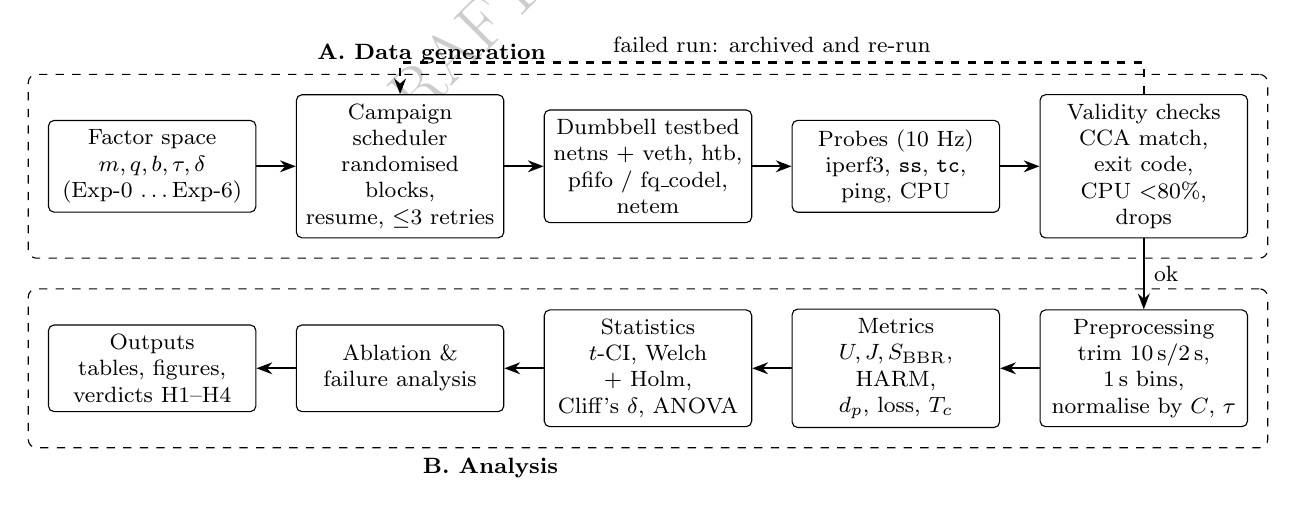
\begin{tikzpicture}[
  font=\footnotesize, node distance=4mm and 5mm,
  box/.style={draw, rounded corners=2pt, align=center, minimum height=11mm, text width=24mm, fill=white},
  grp/.style={draw, dashed, rounded corners=3pt, inner sep=2.5mm},
  arr/.style={-{Stealth[length=2mm]}, thick}]
\node[box] (factors) {Factor space\\$m,q,b,\tau,\delta$\\(Exp-0 \dots Exp-6)};
\node[box, right=of factors] (sched) {Campaign scheduler\\randomised blocks,\\resume, $\le$3 retries};
\node[box, right=of sched] (tb) {Dumbbell testbed\\netns + veth, htb,\\pfifo / fq\_codel, netem};
\node[box, right=of tb] (probe) {Probes (10~Hz)\\iperf3, \texttt{ss}, \texttt{tc},\\ping, CPU};
\node[box, right=of probe] (valid) {Validity checks\\CCA match, exit code,\\CPU $<$80\%, drops};
\node[box, below=9mm of valid] (pre) {Preprocessing\\trim 10\,s/2\,s, 1\,s bins,\\normalise by $C$, $\tau$};
\node[box, left=of pre] (feat) {Metrics\\$U, J, \SB$, HARM,\\$d_{p}$, loss, $T_c$};
\node[box, left=of feat] (stats) {Statistics\\$t$-CI, Welch + Holm,\\Cliff's $\delta$, ANOVA};
\node[box, left=of stats] (abl) {Ablation \&\\failure analysis};
\node[box, left=of abl] (outn) {Outputs\\tables, figures,\\verdicts H1--H4};
\draw[arr] (factors) -- (sched);
\draw[arr] (sched) -- (tb);
\draw[arr] (tb) -- (probe);
\draw[arr] (probe) -- (valid);
\draw[arr] (valid) -- node[right, align=left] {ok} (pre);
\draw[arr] (pre) -- (feat);
\draw[arr] (feat) -- (stats);
\draw[arr] (stats) -- (abl);
\draw[arr] (abl) -- (outn);
\draw[arr, dashed] (valid.north) -- ++(0,4mm) -| node[pos=0.25, above] {failed run: archived and re-run} (sched.north);
\begin{scope}[on background layer]
\node[grp, fit=(factors)(sched)(tb)(probe)(valid), label={[font=\footnotesize\bfseries]above left:A. Data generation}] {};
\node[grp, fit=(pre)(feat)(stats)(abl)(outn), label={[font=\footnotesize\bfseries]below left:B. Analysis}] {};
\end{scope}
\end{tikzpicture}
\caption{Methodology architecture. Block A generates validated runs; block B turns them into metrics, statistical tests and the paper's tables and figures. Failed runs are archived and repeated rather than discarded.}
\label{fig:arch}
\end{figure*}

\subsection{Testbed module}
The dumbbell (Fig.~\ref{fig:topo}) is built from Linux network namespaces connected by veth pairs on a single host, so that all components share one clock. Each sender group $i$ runs in its own namespace with the \texttt{fq} queue discipline for pacing~\cite{bless2025bbrv3}. The router's egress towards the receiver is shaped by \texttt{htb} to $C=100$~Mbit/s, with a child queue of either \texttt{pfifo} (FIFO) or \texttt{fq\_codel} with the \emph{same packet limit}, so that only the queue discipline differs. The buffer limit is $L=\max(2,\lceil b\cdot C\,\tau_{\max}/(8\cdot1500)\rfloor)$ packets, where $\tau_{\max}$ is the longest base RTT in the cell. Propagation delay is added with \texttt{netem}~\cite{hemminger2005netem} on the router's sender-facing egress, i.e.\ the ACK path, so that \texttt{netem}'s own queue never holds data packets. TSO, GSO and GRO are disabled on all veth interfaces to avoid burst artefacts, and \texttt{tcp\_no\_metrics\_save} prevents cached state from leaking between runs.

\begin{figure}[t]
\centering
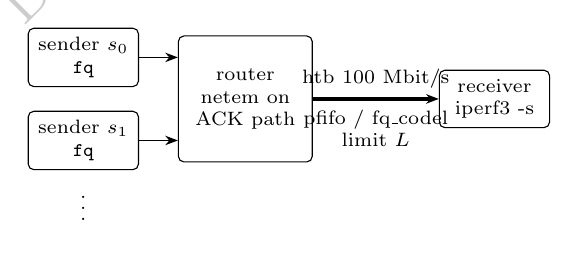
\begin{tikzpicture}[font=\scriptsize, node distance=5mm and 7mm,
  host/.style={draw, rounded corners=2pt, align=center, minimum width=14mm, minimum height=7mm},
  arr/.style={-{Stealth[length=1.6mm]}}]
\node[host] (s0) {sender $s_0$\\\texttt{fq}};
\node[host, below=3mm of s0] (s1) {sender $s_1$\\\texttt{fq}};
\node[below=0mm of s1] (sd) {$\vdots$};
\node[host, right=12mm of $(s0)!0.5!(s1)$, minimum height=16mm, minimum width=17mm] (r) {router\\netem on\\ACK path};
\node[host, right=16mm of r] (rcv) {receiver\\iperf3 -s};
\draw[arr] (s0.east) -- (r.west |- s0.east);
\draw[arr] (s1.east) -- (r.west |- s1.east);
\draw[arr, very thick] (r) -- node[above, align=center] {htb 100 Mbit/s}
  node[below, align=center] {pfifo / fq\_codel\\limit $L$} (rcv);
\end{tikzpicture}
\caption{Dumbbell testbed. Each sender group has its own namespace and base RTT; the single bottleneck is the router's egress to the receiver.}
\label{fig:topo}
\end{figure}

\subsection{Metrics}
Let $x_i(t)$ be the goodput of flow $i$ in 1-s bin $t$, measured by iperf3~\cite{iperf3}, and let $W=[t_a,t_b)$ be the steady-state window. With $\bar{x}_i=|W|^{-1}\sum_{t\in W}x_i(t)$, $N$ flows, the set $\mathcal{B}$ of BBR flows and capacity $C$, the paper uses:
\begin{align}
U &= \frac{1}{C}\sum_{i=1}^{N}\bar{x}_i, \qquad
J = \frac{\left(\sum_i \bar{x}_i\right)^2}{N\sum_i \bar{x}_i^2}, \label{eq:uj}\\
\SB &= \frac{\sum_{i\in\mathcal{B}}\bar{x}_i}{\sum_{i}\bar{x}_i}, \qquad F=\frac{|\mathcal{B}|}{N}, \label{eq:share}\\
h_c &= \max\!\left(0,\ \frac{C/N-\bar{x}_c}{C/N}\right), \label{eq:harm}
\end{align}
where $U$ is utilisation, $J$ is Jain's index~\cite{jain1984fairness}, $\SB$ is the BBR share with fair reference $F$, and $h_c$ is the harm~\cite{ware2019harm} suffered by the mean flow $\bar{x}_c$ of CCA $c$ relative to its equal share. Queuing delay is derived from the bottleneck backlog $B(t)$ in bytes, sampled at 10~Hz, as $d(t)=8B(t)/C(t)$; $\dq{50}$, $\dq{95}$ and $\dq{99}$ denote its percentiles over $W$. Latency under load is the 95th percentile of a 10-Hz ping probe, $\mathrm{RTT}_{95}$. Loss is reported as the qdisc drop rate (drops over drops plus transmitted packets) and as the TCP retransmission rate (retransmitted segments over $\text{bytes}/\text{MSS}$). Stability is captured by the oscillation amplitude $\sigma_S$, the standard deviation of the per-second BBR share, and the mechanism of~\cite{scherrer2026control} by the median ratio of BBR's minimum-RTT estimate to the base RTT. For an event at time $t_e$ (capacity step, RTT step or flow arrival), the convergence time of a series $z(t)$ to threshold $\gamma$ is
\begin{equation}
T(z,\gamma) = \min\{t\ge t_e : z(s)\ge\gamma\ \ \forall s\in[t,t+5)\} - t_e, \label{eq:conv}
\end{equation}
with $T_U=T(U,0.9)$ and $T_J=T(J,0.9)$; $\bar{U}_{10}$ is the mean utilisation over the 10~s after the event.

\subsection{Statistical model and objective}
\label{sec:stats}
The quantity of interest is the interaction between the CCA mix and the queue. It is estimated as a difference-in-differences against the homogeneous reference cells (CUBIC-only and BBR-only):
\begin{equation}
\Delta_{\mathrm{int}}(Y) = \big[\bar{Y}_{\mathrm{mix}}^{\mathrm{FQ}} - \bar{Y}_{\mathrm{mix}}^{\mathrm{FIFO}}\big] - \big[\bar{Y}_{\mathrm{hom}}^{\mathrm{FQ}} - \bar{Y}_{\mathrm{hom}}^{\mathrm{FIFO}}\big]. \label{eq:did}
\end{equation}
Across the regime sweep, each metric is modelled as
\begin{equation}
Y_{qbrk} = \mu + \alpha_q + \beta_b + \gamma_r + (\alpha\beta)_{qb} + (\alpha\gamma)_{qr} + (\beta\gamma)_{br} + (\alpha\beta\gamma)_{qbr} + \varepsilon_{qbrk}, \label{eq:anova}
\end{equation}
where $\alpha_q$, $\beta_b$ and $\gamma_r$ are the queue, buffer and RTT effects, $k$ indexes repetitions and $\varepsilon$ is the residual. Effects are tested with a type-II ANOVA and reported with partial $\eta^2_p = SS_{\mathrm{effect}}/(SS_{\mathrm{effect}}+SS_{\mathrm{res}})$; a rank-transform ANOVA~\cite{conover1981rank} checks robustness to non-normal residuals. Pairwise FIFO vs FQ-CoDel comparisons use Welch's $t$-test~\cite{welch1947} with Holm correction~\cite{holm1979} and Cliff's $\delta$~\cite{cliff1993} as effect size. Means are reported with 95\% Student-$t$ confidence intervals. Practical-significance thresholds were fixed before the experiments: $|\Delta J|\ge0.05$, $|\Delta\dq{95}|\ge5$~ms and $|\Delta U|\ge0.02$.

\subsection{Algorithms}
Algorithm~\ref{alg:campaign} gives the campaign procedure, and Algorithm~\ref{alg:run} a single run with its validity checks.

\begin{algorithm}[t]
\caption{Campaign execution}
\label{alg:campaign}
\begin{algorithmic}[1]
\Require profile $P$ (cells $\mathcal{C}_e$ and repetitions $n_e$ per experiment $e$)
\For{$r = 0$ \textbf{to} $\max_e n_e - 1$}
  \State $\mathcal{K} \gets \{(c,r) : c\in\mathcal{C}_e,\ r<n_e\}$
  \State shuffle $\mathcal{K}$ with seed $1000+r$ \Comment{randomised block}
  \For{$(c,r)\in\mathcal{K}$}
    \If{run $(c,r)$ already valid} \textbf{continue} \Comment{resume}
    \EndIf
    \For{attempt $=1$ \textbf{to} 3}
      \State archive any previous attempt; $s\gets$ \Call{Run}{$c,r$}
      \State log $(c,r,\text{attempt},s)$; idle 5~s
      \If{$s=\textsc{ok}$} \textbf{break}
      \EndIf
    \EndFor
  \EndFor
\EndFor
\end{algorithmic}
\end{algorithm}

\begin{algorithm}[t]
\caption{\textsc{Run}$(c,r)$: one validated run}
\label{alg:run}
\begin{algorithmic}[1]
\State build namespaces, veth links, htb + queue $q$ (limit $L$), netem delays, sender \texttt{fq}
\State measure idle base RTT per group (20 pings, minimum)
\State start iperf3 servers, samplers (\texttt{ss}, \texttt{tc} at 10~Hz; CPU at 2~Hz) and ping probe
\State launch each sender group at its start time with CCA $c_g$; apply scheduled events (rate / RTT changes)
\State wait for all clients; tear down the topology
\State $\text{ok}\gets$ (iperf3 exit codes $=0$) $\wedge$ (CCA seen in \texttt{ss} $=$ requested CCA) $\wedge$ (CPU p95 $<80\%$)
\State flag (not fail) sender-qdisc drops; store raw traces and metadata
\State \Return ok
\end{algorithmic}
\end{algorithm}

\subsection{Changes with respect to the Phase~2 design}
The implementation differs from the Phase~2 methodology in seven documented respects. (i) The ``FQ-only'' ablation uses \texttt{fq\_codel} with CoDel effectively disabled (target 4~s, interval 8~s) instead of \texttt{tc fq}, so that FQ-only and FQ-CoDel share an identical scheduler and hash function and differ only in CoDel. (ii) HARM is computed against the equal share $C/N$ (Eq.~\ref{eq:harm}) rather than against solo runs; homogeneous runs are still reported as references and used in Eq.~\ref{eq:did}. (iii) A ping probe replaces \texttt{irtt}. (iv) To fit the time budget, the number of repetitions is \R{reps-exp1} for the core experiment and \R{reps-exp2}--\R{reps-exp5} elsewhere instead of ten everywhere, and Student-$t$ intervals replace bootstrap intervals, which are unreliable at such sample sizes. (v) The rank-transform ANOVA~\cite{conover1981rank} replaces the aligned rank transform~\cite{wobbrock2011art} as the robustness check. (vi) The steady-state model baseline (B3) and (vii) the BBRv3 ablation (A6), which requires a custom kernel, were deferred; the scripts support A6 through a tagged campaign.

% =========================================================================
\section{Experimental Setup}
\label{sec:setup}

\subsection{Dataset}
No public dataset covers the factor space, so the data were generated on the testbed, following the practice of~\cite{sarpkaya2025sharing,bless2025bbrv3,sarpkaya2025l4s,scherrer2026control}. Table~\ref{tab:exps} lists the seven experiments; together they comprise \R{ncells} cells and \R{nruns} valid runs. Each run directory holds the iperf3 JSON output, 10-Hz \texttt{ss} and \texttt{tc} samples, ping output, CPU samples and a metadata file with all factor levels, tool versions and validity-check results. The dataset is released with the code.

\begin{table}[t]
\centering
\caption{Experiments. Unless stated otherwise: 100 Mbit/s, 50 ms, 2 BDP, 60 s runs (90 s for transients).}
\label{tab:exps}
\footnotesize
\begin{tabular}{@{}p{12mm}p{40mm}cc@{}}
\toprule
Exp. & Factors varied & Cells & Runs/cell \\
\midrule
Exp-0 & Replications of~\cite{sarpkaya2025l4s} (1:1, 10 ms, 2 BDP) and~\cite{kumari2025cubic} (5 CUBIC at 10 ms + 5 at 50 ms, 1000 pkts) $\times$ 2 queues & \R{ncells-exp0} & \R{reps-exp0} \\
Exp-1 & \{CUBIC-only, BBR-only, 1:1\} $\times$ 2 queues & \R{ncells-exp1} & \R{reps-exp1} \\
Exp-2 & 1:1 $\times$ 2 queues $\times$ \{0.5, 1, 2, 4, 8\} BDP $\times$ \{10, 50, 100\} ms & \R{ncells-exp2} & \R{reps-exp2} \\
Exp-3 & \{1:4, 2:2, 4:4, 8:8, 4:1\} $\times$ 2 queues $\times$ \{1, 4\} BDP & \R{ncells-exp3} & \R{reps-exp3} \\
Exp-4 & CUBIC/BBR at 10/50 ms and 50/10 ms $\times$ 2 queues $\times$ \{1, 4\} BDP & \R{ncells-exp4} & \R{reps-exp4} \\
Exp-5 & \{capacity 100$\to$50$\to$100, RTT 20$\to$60 ms, BBR late, CUBIC late\} $\times$ 2 queues & \R{ncells-exp5} & \R{reps-exp5} \\
Exp-6 & 9 ablation variants $\times$ \{1:1, 4:4\} $\times$ \{1, 4\} BDP & \R{ncells-exp6} & \R{reps-exp6} \\
\bottomrule
\end{tabular}
\end{table}

\subsection{Preprocessing and data splits}
For steady-state metrics, the first 10~s (slow start and BBR Startup) and the last 2~s are discarded. In late-join cells the window starts 10~s after the last arrival, and in step cells it ends at the first event. All series are binned to 1~s and aligned on the common host clock. Throughput is normalised by the current capacity and RTT by the measured idle base RTT. Because the study fits no learned model, there is no train/test split; instead, repetitions are independent samples of each cell, and Exp-0 serves as a separate validation set against published settings rather than as part of the hypothesis tests. Runs failing a validity check are archived and repeated, never silently discarded; \R{failattempts} of \R{attempts} attempts failed and were repeated.

\subsection{Baselines}
Three baselines from the Phase~2 design are used: (B1) homogeneous CUBIC-only and BBR-only runs under each queue, which separate inter-protocol from intra-protocol effects; (B2) FIFO tail-drop at the same packet limit, the status-quo queue against which FQ-CoDel is judged; and (B4) the replication settings of Exp-0, which validate the testbed against published observations.

\subsection{Implementation details and environment}
The testbed comprises five Python modules (topology, run control, campaign, metrics, paper assets). Table~\ref{tab:params} lists all parameters. Experiments ran on \R{os} with kernel \R{kernel}, which provides BBRv1 as \texttt{tcp\_bbr}, on a \R{cpu} with \R{ncpu} logical cores and \R{ram}~GB of RAM, using iperf3 \R{iperf} and iproute2 \R{iproute}. The analysis used Python \R{python}, pandas \R{pandas}, NumPy \R{numpy}, SciPy \R{scipy}, statsmodels \R{statsmodels} and Matplotlib \R{matplotlib}. Run order is randomised with seeds $1000+r$ for repetition block $r$. The highest per-run 95th-percentile CPU load was \R{cpu-p95-max}\%, well below the 80\% validity limit, and the measured base RTT deviated from the configured value by \R{rtt-err}~ms in the median (maximum \R{rtt-err-max}~ms).

\begin{table}[t]
\centering
\caption{Testbed parameters (hyperparameters).}
\label{tab:params}
\footnotesize
\resizebox{\columnwidth}{!}{%
\begin{tabular}{@{}ll@{}}
\toprule
Parameter & Value \\
\midrule
Bottleneck rate $C$ & 100 Mbit/s (htb, quantum 60\,000 B) \\
MTU / MSS & 1500 B / 1448 B \\
Buffer limit $L$ & $b\times$BDP packets of 1500 B, BDP at longest base RTT \\
FQ-CoDel & target 5 ms, interval 100 ms, no ECN, memory limit 64 MiB \\
CoDel only / FQ only & target 5 ms / target 4 s, interval 8 s \\
Sender queue & \texttt{fq} (pacing); \texttt{pfifo} in A7 \\
Host TCP & \texttt{tcp\_ecn}=2 (1 in A4), rmem/wmem max 64 MiB \\
Offloads & TSO/GSO/GRO off on all veths \\
Run length & 60 s static, 90 s transient; 5 s idle gap \\
Trim & first 10 s, last 2 s \\
Sampling & \texttt{ss}, \texttt{tc} and ping at 10 Hz; CPU at 2 Hz \\
Validity & iperf3 exit 0, CCA match, CPU p95 $<$80\%; $\le$3 attempts \\
Seeds & run order: \texttt{random.Random(1000+r)} \\
\bottomrule
\end{tabular}}
\end{table}

% =========================================================================
\section{Results and Analysis}
\label{sec:results}

\subsection{Testbed validation}
Table~\ref{tab:validation} reports the two replication settings. In the setting of~\cite{sarpkaya2025l4s}, the harm criterion used there (a flow receiving less than 20\% or more than 80\% of the link) was met in \R{val8-harm-fifo} FIFO runs and \R{val8-harm-fq_codel} FQ-CoDel runs, and the BBR share was \R{val8-share-fifo}\% under FIFO and \R{val8-share-fq_codel}\% under FQ-CoDel. In the RTT-unfairness setting of~\cite{kumari2025cubic}, the ratio of mean per-flow throughput of the 10-ms to the 50-ms CUBIC flows was \R{val7-ratio-fifo} under FIFO and \R{val7-ratio-fq_codel} under FQ-CoDel, with 95th-percentile queuing delay of \R{val7-d95-fifo}~ms and \R{val7-d95-fq_codel}~ms, respectively. Section~\ref{sec:compare} discusses these values against the published observations. \R{flag-util} static runs fell below 90\% utilisation and \R{flag-sdrops} runs recorded drops at a sender queue; both are flagged in the dataset.

\begin{table}[t]
\centering
\caption{Exp-0: replication settings (mean $\pm$ 95\% CI). The sixth column is the BBR share for~\cite{sarpkaya2025l4s} and the per-flow throughput ratio of 10-ms to 50-ms flows for~\cite{kumari2025cubic}. ``Harm'' counts runs with a flow below 20\% or above 80\% of the link.}
\label{tab:validation}
\resizebox{\columnwidth}{!}{\gtab{tab_validation}}
\end{table}

\subsection{Core interaction (Exp-1)}
Table~\ref{tab:core} and Fig.~\ref{fig:core} summarise the core $2\times2$ experiment over $n=\R{e1-n}$ runs per cell. For one CUBIC and one BBR flow, replacing FIFO with FQ-CoDel changed Jain's index from \R{e1-jfi-fifo-ci} to \R{e1-jfi-fq-ci} (Holm-adjusted \R{e1-jfi-p}, Cliff's $\delta=\R{e1-jfi-cd}$), a change that is \R{e1-jfi-sig}. The BBR share moved from \R{e1-share-fifo}\% to \R{e1-share-fq}\% (\R{e1-share-p}); under FIFO \R{e1-dom-fifo} obtained the larger share, and under FQ-CoDel \R{e1-dom-fq} did. The 95th-percentile queuing delay changed from \R{e1-d95-fifo-ci}~ms to \R{e1-d95-fq-ci}~ms (\R{e1-d95-p}, $\delta=\R{e1-d95-cd}$), a FIFO-to-FQ-CoDel ratio of \R{e1-d95-ratio}; this difference is \R{e1-d95-sig}. Latency under load followed: the probe's $\mathrm{RTT}_{95}$ changed from \R{e1-ping95-fifo}~ms to \R{e1-ping95-fq}~ms (\R{e1-ping95-p}). Utilisation changed by \R{e1-util-dpp} percentage points (\R{e1-util-p}), which is \R{e1-util-sig}. The qdisc drop rate was \R{e1-drop-fifo}\% under FIFO and \R{e1-drop-fq}\% under FQ-CoDel, and the retransmission rate \R{e1-retx-fifo}\% and \R{e1-retx-fq}\%.

The homogeneous references isolate the part of these changes that is specific to the mixed population. By Eq.~\eqref{eq:did}, the interaction effect was $\Delta_{\mathrm{int}}(J)=\R{e1-did-jfi}$, $\Delta_{\mathrm{int}}(\dq{95})=\R{e1-did-d95}$~ms and $\Delta_{\mathrm{int}}(U)=\R{e1-did-util}$. A non-zero $\Delta_{\mathrm{int}}$ indicates that the queue discipline affects the mixed population differently from either homogeneous population, which is the interaction the research question asks about.

Fig.~\ref{fig:tscore} shows a qualitative example. The left panels plot the per-algorithm throughput and the queuing delay of one run under each queue; the right panel gives the distribution of the probe RTT over all repetitions. The oscillation amplitude of the BBR share was \R{e1-osc-fifo} under FIFO and \R{e1-osc-fq} under FQ-CoDel (\R{e1-osc-p}).

\begin{table*}[t]
\centering
\caption{Exp-1: core $2\times2$ results at 2 BDP and 50 ms (mean $\pm$ 95\% CI). $d_{95}$: 95th-percentile queuing delay; RTT$_{95}$: 95th-percentile probe RTT under load.}
\label{tab:core}
\resizebox{\textwidth}{!}{\gtab{tab_core}}
\end{table*}

\begin{figure*}[t]
\centering
\gfig{fig_core}{\textwidth}
\caption{Exp-1: utilisation, Jain's index, 95th-percentile queuing delay and retransmission rate for homogeneous and mixed populations under FIFO and FQ-CoDel (error bars: 95\% CI).}
\label{fig:core}
\end{figure*}

\begin{figure*}[t]
\centering
\gfig{fig_ts_core}{\textwidth}
\caption{Exp-1, one CUBIC and one BBR flow. Left and centre: per-algorithm throughput (solid) and queuing delay (dotted, right axis) of one run. Right: CDF of the probe RTT under load over all repetitions (seconds 10--58).}
\label{fig:tscore}
\end{figure*}

\subsection{Buffer and RTT regimes (Exp-2)}
Fig.~\ref{fig:regime} maps the BBR share and $\dq{95}$ over the buffer--RTT plane, and Table~\ref{tab:regime} in the Appendix gives Jain's index, utilisation and drop rate for every cell. \R{h1-sentence}. H1 is therefore \R{h1-verdict}. Under FIFO, the smallest buffer at which CUBIC held the majority of the capacity on average was \R{h1-cross}~BDP. The worst-case cell means were $J=\R{e2-jfi-min-fifo}$ for FIFO and $J=\R{e2-jfi-min-fq_codel}$ for FQ-CoDel, and the largest mean $\dq{95}$ was \R{e2-d95-max-fifo}~ms for FIFO and \R{e2-d95-max-fq_codel}~ms for FQ-CoDel.

For the deep-buffer configurations ($\ge$2~BDP), the FIFO-to-FQ-CoDel ratio of $\dq{95}$ had a median of \R{h4-ratio-med} and a minimum of \R{h4-ratio-min}, and the largest utilisation loss was \R{h4-uloss-max} percentage points; \R{h4-nok} of \R{h4-ncells} configurations met both parts of the H4 criterion, so H4 is \R{h4-verdict}.

Table~\ref{tab:anova} quantifies these effects with the factorial model of Eq.~\eqref{eq:anova}. The queue main effect explained $\eta^2_p=\R{anova-q-J-eta}$ of the variance in $J$ (\R{anova-q-J-p}), $\R{anova-q-S-eta}$ in $\SB$ (\R{anova-q-S-p}) and $\R{anova-q-D-eta}$ in $\log\dq{95}$ (\R{anova-q-D-p}). The queue$\times$buffer interaction reached $\eta^2_p=\R{anova-qb-S-eta}$ for $\SB$ (\R{anova-qb-S-p}) and the queue$\times$RTT interaction $\eta^2_p=\R{anova-qr-S-eta}$ (\R{anova-qr-S-p}). The residuals \R{anova-shapiro-word} normality (smallest Shapiro--Wilk \R{anova-shapiro-min}); the rank-transform ANOVA agreed with the parametric one on the significance of \R{anova-agree} of \R{anova-total} terms.

Fig.~\ref{fig:mech} tests the mechanism proposed by~\cite{scherrer2026control}. The mean BBR minimum-RTT inflation reached \R{mech-mrtt-max-fifo}$\times$ the base RTT under FIFO and \R{mech-mrtt-max-fq_codel}$\times$ under FQ-CoDel, and across FIFO runs its rank correlation with the BBR share was $\rho=\R{mech-rho}$ (\R{mech-p}). The mean oscillation amplitude was \R{mech-osc-fifo} under FIFO and \R{mech-osc-fq_codel} under FQ-CoDel.

\begin{figure}[t]
\centering
\gfig{fig_regime}{\columnwidth}
\caption{Exp-2 regime maps (mean over repetitions): BBR throughput share (top; 50\% is the fair share) and 95th-percentile queuing delay (bottom, log colour scale) over buffer size and base RTT.}
\label{fig:regime}
\end{figure}

\begin{table*}[t]
\centering
\caption{Exp-2: factorial ANOVA (type II) of the regime sweep. $\eta^2_p$: partial eta squared. Queuing delay is log-transformed because of its skew.}
\label{tab:anova}
\footnotesize
\gtab{tab_anova}
\end{table*}

\begin{figure}[t]
\centering
\gfig{fig_mech}{\columnwidth}
\caption{Exp-2 mechanism indicators versus buffer size (pooled over RTT, 95\% CI): BBR's minimum-RTT estimate relative to the base RTT (left) and the oscillation amplitude of the BBR share (right).}
\label{fig:mech}
\end{figure}

\subsection{Flow-count scaling (Exp-3)}
Table~\ref{tab:flows} and Fig.~\ref{fig:flows} extend the mix to 16 flows and to unequal populations. The largest mean deviation of the BBR share from its fair share was \R{e3-excess-max-fifo} percentage points under FIFO and \R{e3-excess-max-fq_codel} under FQ-CoDel, and the lowest mean Jain index was \R{e3-jfi-min-fifo} and \R{e3-jfi-min-fq_codel}, respectively. With eight flows of each algorithm, the setting in which~\cite{ahsan2026bbrn} reported degrading fairness, FQ-CoDel achieved $J=\R{e3-jfi-8-fq_codel-b1}$ at 1~BDP and $J=\R{e3-jfi-8-fq_codel-b4}$ at 4~BDP, against \R{e3-jfi-8-fifo-b1} and \R{e3-jfi-8-fifo-b4} under FIFO.

\begin{table}[t]
\centering
\caption{Exp-3: flow scaling at 50 ms (means). C:B = CUBIC:BBR flows; $F$ = fair BBR share; $S_\mathrm{BBR}$ in \%, $d_{95}$ in ms.}
\label{tab:flows}
\resizebox{\columnwidth}{!}{\gtab{tab_flows}}
\end{table}

\begin{figure}[t]
\centering
\gfig{fig_flows}{\columnwidth}
\caption{Exp-3: deviation of the BBR share from its fair share (percentage points; positive = BBR over-shares) for each population at 1 and 4 BDP (95\% CI).}
\label{fig:flows}
\end{figure}

\subsection{RTT heterogeneity (Exp-4)}
Table~\ref{tab:rtt} places the two algorithms on different base RTTs. The lowest mean Jain index across these cells was \R{e4-jfi-min-fifo} under FIFO and \R{e4-jfi-min-fq_codel} under FQ-CoDel. With CUBIC at 10~ms and BBR at 50~ms, the BBR share at 1~BDP was \R{e4-share-c10-fifo-b1}\% under FIFO and \R{e4-share-c10-fq_codel-b1}\% under FQ-CoDel; with the RTTs reversed, it was \R{e4-share-c50-fifo-b1}\% and \R{e4-share-c50-fq_codel-b1}\%. Because FQ-CoDel schedules packets rather than RTT-weighted windows, it is expected to remove the RTT bias that FIFO inherits from window-based sharing; these values quantify how far that holds for a mixed CCA population.

\begin{table}[t]
\centering
\caption{Exp-4: RTT heterogeneity (means; $S_\mathrm{BBR}$ with 95\% CI). The BDP is computed at the longer RTT.}
\label{tab:rtt}
\resizebox{\columnwidth}{!}{\gtab{tab_rtt}}
\end{table}

\subsection{Transient behaviour (Exp-5)}
Table~\ref{tab:transient} reports convergence after each event, and Fig.~\ref{fig:transient} shows one run per scenario. When capacity was restored from 50 to 100~Mbit/s, aggregate utilisation converged after \R{e5-capconv-fifo}~s under FIFO and \R{e5-capconv-fq_codel}~s under FQ-CoDel. In the 10~s after the RTT increase, utilisation fell short of the link by \R{e5-rttdip-fifo}\% under FIFO and \R{e5-rttdip-fq_codel}\% under FQ-CoDel. Per algorithm, \R{h3-sentence}; H3 is therefore \R{h3-verdict}. For late arrivals, the steady-state BBR share after a late BBR flow joined was \R{e5-share-bbrlate-fifo}\% (FIFO) and \R{e5-share-bbrlate-fq_codel}\% (FQ-CoDel), and after a late CUBIC flow joined \R{e5-share-cubiclate-fifo}\% and \R{e5-share-cubiclate-fq_codel}\%, which indicates whether the incumbent kept an advantage of the kind reported for BBRv3 in~\cite{mahmud2026startup}.

\begin{table}[t]
\centering
\caption{Exp-5: transient metrics (mean $\pm$ 95\% CI). $T_U$, $T_J$: time to $U\ge0.9$ and $J\ge0.9$ for 5 s (Eq.~\ref{eq:conv}); superscript $(k/n)$: only $k$ of $n$ runs converged; n.c.: none converged. $\bar U_{10}$: mean utilisation over 10 s after the event.}
\label{tab:transient}
\resizebox{\columnwidth}{!}{\gtab{tab_transient}}
\end{table}

\begin{figure*}[t]
\centering
\gfig{fig_transient}{\textwidth}
\caption{Exp-5 examples (one run each): per-algorithm throughput (solid), capacity (dashed) and queuing delay (dotted, right axis) for the capacity step, the RTT step and a late-joining BBR flow. Vertical lines mark events.}
\label{fig:transient}
\end{figure*}

% =========================================================================
\section{Comparison with Base Papers and State of the Art}
\label{sec:compare}

\subsection{Summary of the base papers}
The research problem was derived from three base papers~\cite{ahsan2026bbrn,han2026bbres,abrol2026survey}; the experimental design additionally builds on two studies whose settings were replicated~\cite{kumari2025cubic,sarpkaya2025l4s}. Table~\ref{tab:base} summarises them.

\begin{table*}[t]
\centering
\caption{Base papers and replication anchors. Reported results are as stated by the authors.}
\label{tab:base}
\scriptsize
\setlength{\tabcolsep}{3pt}
\begin{tabular}{@{}p{21mm}p{23mm}p{25mm}p{21mm}p{17mm}p{30mm}p{24mm}@{}}
\toprule
Paper & Problem & Method & Dataset / platform & Metrics & Reported results & Key limitations \\
\midrule
Ahsan \& Hussain, 2026~\cite{ahsan2026bbrn} & BBRv3 latency and throughput under modern AQMs & BBR-n+ (``smart exit'') vs BBRv3, CUBIC under FQ-CoDel, CAKE & Wired and Wi-Fi testbed, iPerf3/Flent & Throughput, HTTP delay, ping, fairness & $\approx$15--20\% throughput over BBRv3; ping 17\% (vs BBRv3), 45\% (vs CUBIC) better; fairness vs CUBIC degrades at $\ge$8 streams & FIFO baseline under-tested; narrow RTT/buffer range; medians only \\
Han \& Hasegawa, 2026~\cite{han2026bbres} & BBR RTT fairness and stability & BBR-ES: extra state, trend-based transitions & Mininet + Amazon EC2 paths & Jain index, utilisation, queuing delay & $J>0.9$, $U>98\%$ in most settings; bounded delay & AQM not varied; loss and latency-under-load secondary \\
Abrol et al., 2026~\cite{abrol2026survey} & State of BBR research & Survey and taxonomy of BBRv1--v3 & Literature corpus & Qualitative trade-offs & Persistent BBR--CUBIC unfairness, shallow-buffer loss, bufferbloat & No measurements; no unified cross-AQM benchmark \\
Kumari et al., 2025~\cite{kumari2025cubic} & CUBIC under FQ-AQMs in steady and transient states & FIFO vs FQ-CoDel vs FQ-PIE (RFC 9743 scenarios) & ns-3 dumbbell, OpenWRT AP & Throughput, queue delay, HARM & FIFO 578 ms delay; FQ-CoDel $\approx$5 s to reclaim capacity, $\approx$18\% loss after RTT rise & No BBR; default parameters; mainly simulation \\
Sarpkaya et al., 2025~\cite{sarpkaya2025l4s} & L4S CCAs in partial deployment & 9 queue types $\times$ 0.5--8 BDP & FABRIC, 100 Mbit/s, 10 ms & Throughput share, delay, harm & Only flow-isolating queues give fair shares & One network setting; L4S focus \\
\bottomrule
\end{tabular}
\end{table*}

\subsection{Quantitative comparison}
Table~\ref{tab:quant} places the measurements of this study next to the values reported in the base papers. Reported values are marked with an asterisk and are taken from the original publications; no base-paper algorithm was re-implemented, because BBR-n+ and BBR-ES require kernels that are not publicly packaged. All values of this work were measured on the stock Linux BBR (v1) and CUBIC implementations.

\begin{table*}[t]
\centering
\caption{Quantitative comparison with the base papers. $^{*}$Value reported in the cited paper (not re-measured). ``Match'' rates how closely the settings correspond: \textbf{S} = same setting replicated, \textbf{P} = partially comparable, \textbf{D} = different question.}
\label{tab:quant}
\footnotesize
\setlength{\tabcolsep}{3pt}
\begin{tabular}{@{}p{24mm}p{47mm}p{30mm}p{55mm}c@{}}
\toprule
Paper & Metric and setting & Reported$^{*}$ & This work (FIFO $\rightarrow$ FQ-CoDel unless stated) & Match \\
\midrule
\cite{ahsan2026bbrn} BBR-n+ & Fairness vs CUBIC with 8 streams each, FQ-CoDel & degrades$^{*}$ & $J=\R{e3-jfi-8-fq_codel-b1}$ (1 BDP), \R{e3-jfi-8-fq_codel-b4} (4 BDP) & P \\
\cite{ahsan2026bbrn} BBR-n+ & Ping latency improvement (wired) & 45\% vs CUBIC$^{*}$ & RTT$_{95}$ reduction FIFO$\rightarrow$FQ-CoDel: \R{e1-ping-red-pct}\% & D \\
\cite{han2026bbres} BBR-ES & Jain index, mixed traffic & $>0.90^{*}$ & $J=\R{e1-jfi-fq}$; $\Delta=\R{e1-jfi-dabs}$ vs FIFO & P \\
\cite{han2026bbres} BBR-ES & Link utilisation & $>98\%^{*}$ & $U=\R{e1-util-fq}$ (FQ-CoDel), \R{e1-util-fifo} (FIFO) & P \\
\cite{bless2025bbrv3} Bless et al. & Standing queue of BBR-only traffic, drop-tail & $\approx$0.95 RTT$_{\min}$ per flow$^{*}$ & $d_{50}/\tau$ = \R{e1-bbr2-d50norm-fifo} (FIFO), \R{e1-bbr2-d50norm-fq_codel} (FQ-CoDel), 2 BBRv1 flows & P \\
\cite{shrestha2025wifi} Shrestha et al. & Who dominates under FQ-CoDel & BBRv3 dominates$^{*}$ & $\SB=\R{e1-share-fq}$\% (FIFO: \R{e1-share-fifo}\%) & P \\
\cite{kumari2025cubic} Kumari et al. & Time to reclaim capacity, FQ-CoDel & $\approx$5 s$^{*}$ (CUBIC only) & $T_U=\R{e5-capconv-fq_codel}$ s (FIFO \R{e5-capconv-fifo} s), mixed traffic & P \\
\cite{kumari2025cubic} Kumari et al. & Throughput loss after RTT increase, FQ-CoDel & $\approx$18\%$^{*}$ & \R{e5-rttdip-fq_codel}\% (FIFO \R{e5-rttdip-fifo}\%) in first 10 s & P \\
\cite{kumari2025cubic} Kumari et al. & RTT unfairness, 10 vs 50 ms CUBIC & FIFO unfair, FQ fair$^{*}$ & throughput ratio \R{val7-ratio-fifo} $\rightarrow$ \R{val7-ratio-fq_codel} & S \\
\cite{sarpkaya2025l4s} Sarpkaya et al. & Harmed runs, 100 Mbit/s, 10 ms, CUBIC vs BBR & only FQ queues fair$^{*}$ & \R{val8-harm-fifo} $\rightarrow$ \R{val8-harm-fq_codel} runs; $\SB$ \R{val8-share-fifo}\% $\rightarrow$ \R{val8-share-fq_codel}\% & S \\
\cite{scherrer2026control} Scherrer et al. & BBR/CUBIC oscillation, drop-tail & oscillation present$^{*}$ & $\sigma_S$ = \R{mech-osc-fifo} $\rightarrow$ \R{mech-osc-fq_codel} & P \\
\bottomrule
\end{tabular}
\end{table*}

\subsection{Methodological comparison}
The base papers improve coexistence by changing the \emph{sender}: BBR-n+ alters BBRv3's probing exit~\cite{ahsan2026bbrn}, and BBR-ES adds a state and trend-based transitions~\cite{han2026bbres}. This study holds the senders fixed at the deployed Linux implementations and changes only the \emph{bottleneck queue}, varying one factor at a time inside a full factorial design. This difference addresses three limitations of the base papers: the FIFO baseline that~\cite{ahsan2026bbrn} under-tests is a first-class factor here; the AQM dimension that~\cite{han2026bbres} leaves implicit is varied and decomposed into its FQ and CoDel components; and the unified cross-AQM benchmark that~\cite{abrol2026survey} calls for is provided with repeated runs and inferential statistics rather than single medians.

\subsection{Improvement analysis}
Relative to the FIFO baseline in the core setting, FQ-CoDel changed Jain's index by \R{e1-jfi-dabs} in absolute terms (\R{e1-jfi-rel}\% relative), the 95th-percentile queuing delay by \R{e1-d95-rel}\%, and utilisation by \R{e1-util-dpp} percentage points. Measured against the operating point reported for BBR-ES~\cite{han2026bbres} ($J=0.90$, $U=98\%$), the stock senders under FQ-CoDel differed by $\Delta J=\R{cmp2-jfi-abs}$ (\R{cmp2-jfi-rel}\% relative) and $\Delta U=\R{cmp2-util-abs}$ percentage points. Any gain obtained in this way comes from the bottleneck alone: per-flow round-robin scheduling removes the dependence of the throughput split on how aggressively each algorithm fills a shared buffer, and CoDel bounds the per-flow sojourn time. The ablation in Section~\ref{sec:ablation} quantifies how much each of these two mechanisms contributes.

\subsection{Fairness of the comparison and limitations}
The comparison is not like for like in four respects. First, the base papers evaluate BBRv3 or their own variants, whereas this study uses mainline BBRv1, which is known to be more aggressive towards CUBIC in shallow buffers~\cite{hock2017bbr,cao2019bbr}. Second, platforms differ: Wi-Fi in~\cite{shrestha2025wifi}, ns-3 in~\cite{kumari2025cubic}, EC2 paths in~\cite{han2026bbres}, and a single-host emulation here. Third, link rates, RTTs and buffer sizes match only in the two replicated settings (marked S in Table~\ref{tab:quant}). Fourth, several reported values are qualitative and can only be compared in direction. Where this study's FQ-CoDel configuration does not reach a value reported for a modified sender, the difference reflects both the change of sender and the change of platform and cannot be attributed to the queue alone.

% =========================================================================
\section{Ablation Study}
\label{sec:ablation}

Table~\ref{tab:ablation} and Fig.~\ref{fig:ablation} report the nine variants of Exp-6. Each removes, replaces or modifies one component of the FQ-CoDel treatment (A3) or of the sender configuration.

\textbf{Flow isolation versus delay control (A0--A3).} Pooled over the four conditions (1:1 and 4:4 mixes, 1 and 4~BDP), full FQ-CoDel raised Jain's index over FIFO by \R{h2-gain} and reduced $\dq{95}$ by \R{h2-red}~ms. FQ alone (A1) achieved \R{h2-fq-frac}\% of the fairness gain and CoDel alone (A2) \R{h2-codel-fair-frac}\%; CoDel alone achieved \R{h2-codel-frac}\% of the delay reduction and FQ alone \R{h2-fq-del-frac}\%. The ablation therefore identifies \R{h2-fair-src} as the main source of the fairness gain and \R{h2-del-src} as the main source of the delay reduction, and H2 is \R{h2-verdict}. The pooled BBR share exceeded its fair share by \R{abl-excess-a1}~pp under A1 and \R{abl-excess-a3}~pp under A3. Under A3, CoDel's losses fell \R{abl-loss-word} (retransmission rate \R{abl-retxc-a3}\% for CUBIC versus \R{abl-retxb-a3}\% for BBR), which bears directly on the explanation for BBR dominance under FQ-CoDel suggested by~\cite{shrestha2025wifi}.

\textbf{ECN marking (A4).} With ECN enabled at the hosts and the queue, \R{abl-ecn-a4}\% of packets were marked; the retransmission rate changed from \R{abl-retx-a3}\% (A3) to \R{abl-retx-a4}\%, $\dq{95}$ from \R{abl-d95-a3}~ms to \R{abl-d95-a4}~ms, and $J$ from \R{abl-jfi-a3} to \R{abl-jfi-a4}. BBRv1 ignores ECN marks, so only the CUBIC flows respond to them.

\textbf{CoDel target (A5).} Raising the target from 5~ms to 10 and 20~ms changed utilisation from \R{abl-util-a3} to \R{abl-util-a5a} and \R{abl-util-a5b}, and $\dq{95}$ from \R{abl-d95-a3}~ms to \R{abl-d95-a5a}~ms and \R{abl-d95-a5b}~ms. This addresses the question raised in~\cite{kumari2025cubic} of whether the default target is too tight.

\textbf{Sender pacing (A7).} Without the \texttt{fq} queue at the senders, $J$ changed from \R{abl-jfi-a0} to \R{abl-jfi-a7a} under FIFO and from \R{abl-jfi-a3} to \R{abl-jfi-a7b} under FQ-CoDel, and $\dq{95}$ from \R{abl-d95-a0} to \R{abl-d95-a7a}~ms and from \R{abl-d95-a3} to \R{abl-d95-a7b}~ms. These differences indicate how sensitive the conclusions are to the host pacing configuration, which is rarely reported in the literature.

\begin{table*}[t]
\centering
\caption{Exp-6: ablation (means over repetitions). $|S_\mathrm{BBR}-F|$: absolute deviation of the BBR share from its fair share in percentage points.}
\label{tab:ablation}
\footnotesize
\gtab{tab_ablation}
\end{table*}

\begin{figure*}[t]
\centering
\gfig{fig_ablation}{\textwidth}
\caption{Exp-6: Jain's index, deviation from the fair share and 95th-percentile queuing delay (log scale) for each ablation variant at 1 and 4 BDP, pooled over the 1:1 and 4:4 mixes (95\% CI).}
\label{fig:ablation}
\end{figure*}

% =========================================================================
\section{Discussion}
\label{sec:discussion}

\subsection{Why the results take this form}
Under a FIFO queue, the throughput split between CUBIC and BBR is set by how much of the shared buffer each algorithm occupies: CUBIC grows its window until the buffer overflows, while BBR caps its in-flight data at a multiple of its estimated BDP~\cite{ware2019modeling}. Because CUBIC's standing queue also inflates BBR's minimum-RTT estimate~\cite{scherrer2026control}, the split depends on the buffer size and RTT, which is what the queue$\times$buffer and queue$\times$RTT terms in Table~\ref{tab:anova} measure. FQ-CoDel changes both inputs. Its deficit-round-robin scheduler serves backlogged flows in turn, which decouples throughput from buffer occupancy, and CoDel bounds each flow's sojourn time, which limits the standing queue that BBR would otherwise misread as propagation delay. The ablation separates the two: \R{h2-fair-src} accounted for most of the fairness change and \R{h2-del-src} for most of the delay change.

\subsection{Practical implications}
Operators choosing a bottleneck queue for mixed CUBIC/BBR traffic can read Fig.~\ref{fig:regime} directly as a deployment map: each cell shows, for a buffer size and RTT, the share BBR obtains and the delay the queue imposes. In the deep-buffer regime, FQ-CoDel met the delay-reduction criterion in \R{h4-nok} of \R{h4-ncells} configurations at a maximum utilisation cost of \R{h4-uloss-max} percentage points. The transient results in Table~\ref{tab:transient} give the other side of the trade-off: how long each queue needs to restore full utilisation after capacity and RTT increases, which is where a short CoDel-controlled queue can cost throughput.

\subsection{Strengths}
The design varies one factor at a time inside a full factorial, keeps the packet limit identical across queue disciplines, runs the deployed kernel implementations, randomises run order, archives and repeats failed runs, fixes hypotheses and practical thresholds before the experiments, and reports intervals, corrected tests and effect sizes. Every number in this paper is generated by script from the released data.

\subsection{Failure cases}
Table~\ref{tab:failures} applies the failure criteria defined in Phase~2 to every steady-state cell. Under FIFO, \R{fail-harm-fifo} mixed cells gave one algorithm a share outside 0.4--1.6 times its fair share; \R{fail-harm-infl-fifo} of these \R{fail-harm-n-fifo} cells also showed BBR minimum-RTT inflation above 1.25, the signature of the mechanism in~\cite{scherrer2026control}, and \R{fail-harm-shallow-fifo} were shallow-buffer cells in which BBR over-shared, the behaviour reported in~\cite{bless2025bbrv3}. Under FQ-CoDel, \R{fail-harm-fq_codel} mixed cells violated the same criterion. \R{fail-delay-fifo} FIFO cells and \R{fail-delay-fq_codel} FQ-CoDel cells exceeded 100~ms of 95th-percentile queuing delay.

\begin{table}[t]
\centering
\caption{Failure analysis over all steady-state cells of Exp-0 to Exp-4 (cells meeting each criterion / cells evaluated). Share criteria apply to mixed populations only.}
\label{tab:failures}
\footnotesize
\gtab{tab_failures}
\end{table}

\subsection{Limitations and threats to validity}
\emph{Internal validity.} All components share one host, so CPU contention or timer granularity could distort results; the CPU check, disabled offloads, the per-run base-RTT measurement and the Exp-0 replications mitigate this. \emph{External validity.} The study uses a single wired bottleneck at 100~Mbit/s, long-lived bulk flows and BBRv1; results may differ for BBRv3, higher rates, wireless links, short flows and real traffic mixes. \emph{Construct validity.} Jain's index hides the direction of unfairness, so the BBR share and harm are reported alongside it; queuing delay is derived from backlog samples at 10~Hz, which can miss sub-100-ms peaks. \emph{Statistical conclusion validity.} With \R{reps-exp2}--\R{reps-exp1} repetitions per cell, small effects may go undetected; the Holm correction, pre-registered thresholds and the rank-based ANOVA reduce false positives.

\subsection{Were the research gap and objectives met?}
Table~\ref{tab:goals} maps the Phase~1/2 gaps to the evidence. G1 (no controlled, quantified CCA$\times$queue interaction) is addressed by Exp-1 and Exp-2 with Eq.~\eqref{eq:did} and Table~\ref{tab:anova}; G2 (FQ versus CoDel) by Exp-6; G3 (transients with mixed traffic) by Exp-5; and G4 (fragmented metrics and weak statistics) by the unified metric suite and inferential analysis applied to every experiment. The BBRv3 ablation and the steady-state model baseline remain open (Section~\ref{sec:method}).

\begin{table}[t]
\centering
\caption{Research gaps, questions and outcome.}
\label{tab:goals}
\footnotesize
\begin{tabular}{@{}p{9mm}p{36mm}p{12mm}p{15mm}@{}}
\toprule
Gap & Question / hypothesis & Evidence & Outcome \\
\midrule
G1, G4 & RQ1/H1: buffer dependence under FIFO, fairness under FQ-CoDel & Exp-1, 2; Tab.~\ref{tab:anova} & \R{h1-verdict} \\
G2 & RQ2/H2: FQ drives fairness, CoDel drives delay & Exp-6 & \R{h2-verdict} \\
G3 & RQ3/H3: slower FQ-CoDel recovery; BBR faster than CUBIC & Exp-5 & \R{h3-verdict} \\
G4 & RQ4/H4: $\ge$10$\times$ delay reduction at $<$5\% cost & Exp-2 & \R{h4-verdict} \\
\bottomrule
\end{tabular}
\end{table}

% =========================================================================
\section{Conclusion and Future Work}
\label{sec:conclusion}

This paper measured the interaction between TCP CUBIC/BBR and FIFO/FQ-CoDel bottleneck queues in a controlled factorial testbed over \R{nruns} validated runs. In the core setting, FQ-CoDel changed Jain's index from \R{e1-jfi-fifo} to \R{e1-jfi-fq} and the 95th-percentile queuing delay from \R{e1-d95-fifo}~ms to \R{e1-d95-fq}~ms; across the regime sweep, the queue discipline interacted with buffer size and RTT as quantified by the factorial model; and the ablation attributed the fairness change mainly to \R{h2-fair-src} and the delay change mainly to \R{h2-del-src}. The four hypotheses were \R{h1-verdict}, \R{h2-verdict}, \R{h3-verdict} and \R{h4-verdict}, respectively. Future work should repeat the campaign with BBRv3 and with ECN-aware senders, extend it to higher link rates and to physical or wireless bottlenecks, add short and interactive flows, and use the released dataset to build a model of BBR--CUBIC sharing under fair queuing.

% =========================================================================
\section*{Declarations}
\noindent\textbf{Data and code availability.} The testbed, campaign scripts, raw and processed data and the script that generates every table, figure and number in this paper are available at \repourl.

\noindent\textbf{Conflict of interest.} The author declares no conflict of interest.

\noindent\textbf{Funding.} This research received no external funding.

\noindent\textbf{AI-tool usage.} An AI assistant (Claude, Anthropic) was used to help draft and edit the text, prepare the \LaTeX{} source and write the analysis and plotting scripts. The research design, the execution of all experiments, and the verification of all content and results are the author's own; all reported numbers are computed by the released scripts from the experimental data.

\noindent\textbf{Acknowledgements.} The author thanks the Computer Networks course instructor at FAST-NUCES Islamabad for guidance throughout the project.

% =========================================================================
\bibliographystyle{IEEEtran}
\bibliography{refs}

% =========================================================================
\appendices
\section{Per-cell regime results}
Table~\ref{tab:regime} lists Jain's index, utilisation and qdisc drop rate for every cell of Exp-2 (means over repetitions).

\begin{table*}[t]
\centering
\caption{Exp-2: Jain's index, utilisation and drop rate per buffer size, queue and base RTT (means).}
\label{tab:regime}
\footnotesize
\gtab{tab_regime}
\end{table*}

\section{Reproduction}
On Ubuntu 22.04/24.04: \texttt{sudo bash setup\_host.sh}; \texttt{sudo python3 campaign.py --profile paper}; \texttt{python3 metrics.py data}; \texttt{python3 make\_paper\_assets.py data paper/generated}; then compile \texttt{paper/main.tex}. A single cell can be debugged with \texttt{sudo python3 run\_cell.py <cell\_id> <outdir>}, and \texttt{--dry-run} lists the full run plan.

\end{document}
